\documentclass[conference]{IEEEtran}
\usepackage{amsmath,amssymb}
\usepackage{booktabs}
\usepackage{array}
\usepackage{xcolor}
\usepackage{url}
\usepackage{graphicx}
\usepackage{dblfloatfix}
\usepackage{capt-of}
\usepackage{titlesec}

\newcommand{\um}{\ensuremath{\mu\mathrm{m}^2}}
\renewcommand{\thesection}{\arabic{section}}
\renewcommand{\thesubsection}{\thesection.\arabic{subsection}}
\renewcommand{\thesubsubsection}{\thesubsection.\arabic{subsubsection}}
\renewcommand{\thesectiondis}{\thesection}
\renewcommand{\thesubsectiondis}{\thesubsection}
\renewcommand{\thesubsubsectiondis}{\thesubsubsection}
\titleformat{\section}
  {\normalfont\large\bfseries}{\thesection}{1em}{}
\titleformat{\subsection}
  {\normalfont\large\bfseries}{\thesubsection}{0.8em}{}
\titleformat{\subsubsection}
  {\normalfont\normalsize\bfseries}{\thesubsubsection}{0.8em}{}
\titlespacing*{\section}{0pt}{1.6ex plus 0.6ex minus 0.2ex}{0.8ex}
\titlespacing*{\subsection}{0pt}{1.2ex plus 0.4ex minus 0.2ex}{0.6ex}
\titlespacing*{\subsubsection}{0pt}{1.0ex plus 0.3ex minus 0.2ex}{0.4ex}

\title{STDM: A Shared Tangent-Plane FP32 Divider--Multiplier\\
with Multi-Level Accuracy--PPA Tradeoffs}
\author{\IEEEauthorblockN{Pingchuan Dong}
}

\begin{document}
\maketitle

\begin{abstract}
Approximate floating-point division and multiplication are usually designed as
independent operators, even when a processing element issues only one of them
at a time. This paper presents STDM, four FP32 divider--multiplier designs that
share a piecewise tangent-plane mantissa datapath. We prove that local
approximations of multiplication and division use the same two residual terms
and a cell-dependent constant. Reciprocal-square scaling for division is folded
into these coefficients, eliminating a separate post-plane multiplier. We also
introduce an exact unsigned recoding of centered residuals: the operation sign
is absorbed into the selected constant and a bitwise complement of the short
divisor residual. The resulting datapath uses two unsigned products and one
positive accumulation without changing any approximate output. In a TSMC
65-nm implementation, sharing at L1--L3 reduces area by 17.2--19.0\%, power by
31.6--42.4\%, and area--delay product by 11.8--14.4\% relative to matched
separate cores, with at most 6.5\% delay overhead. DIV-only comparisons include
PACE, FPD2D, PLSAD, and other approximate FP32 dividers under a common local
flow. At L3, the complete shared unit reduces area, delay, power, and
area--delay product by 92.5\%, 74.5\%, 98.1\%, and 98.1\%, respectively,
relative to an exact DesignWare FP32 DIV+MUL unit.
\end{abstract}

\begin{IEEEkeywords}
approximate computing, floating-point arithmetic, divider, multiplier,
tangent-plane approximation, arithmetic sharing, ASIC
\end{IEEEkeywords}

\section{Introduction}
Approximate arithmetic reduces the cost of floating-point computation when an
application can tolerate bounded numerical error. Most approximate dividers
and multipliers are nevertheless optimized as independent units. A processing
element that issues one operation at a time then pays for two mantissa
datapaths, even though both operate on the same normalized significands and
share normalization and packing. Avoiding this duplication requires more than
placing two compact operators behind a selector: their approximations must be
expressed in a common arithmetic form.

Prior dividers simplify digit recurrence, reciprocal evaluation, logarithmic
conversion, or a fitted quotient surface. PACE progressively corrects a
piecewise reciprocal~\cite{wen2025pace}; PLSAD and FPD2D show that quantized
local planes can give particularly low-cost DIV-only implementations
\cite{wu2024plsad,dimeo2025fpd2d}. OAM uses midpoint tangent planes for
multiplication~\cite{chen2020oam}. These results establish strong
operator-level tradeoffs, but leave open whether
a planar FP32 divider and multiplier can share their dominant arithmetic
without reducing them to a logarithmic approximation.

STDM answers this question with four fixed-level FP32 divider--multiplier
designs. For a selected cell, let $k_x,k_y$ be its midpoint and let
$r_x=x-k_x$, $r_y=y-k_y$. The multiplier plane is
$k_xk_y+k_yr_x+k_xr_y$, while the divider plane is
$(k_xk_y+k_yr_x-k_xr_y)/k_y^2$. Hence both operations are affine functions of
the same two residuals. STDM folds the reciprocal-square factor into the
divider slopes and constant, so either mode is evaluated as one table-selected
constant plus two products. This avoids both an inter-level correction chain
and a post-plane coefficient multiplier.

The remaining problem is realizing the signed affine form efficiently. STDM
truncates only the low residual bits selected for each level and then applies
an exact unsigned recoding. Adding the residual half-range converts each short
signed residual to an unsigned field. In DIV mode, a bitwise complement of the
$y$ field and a precomputed constant adjustment implement the negative term.
MUL and DIV therefore use the same two unsigned products and one positive
accumulation. This transformation changes circuit organization but not the
computed approximation. Reciprocal coefficients are calibrated using the
complete packed FP32 result before being folded into the slopes and constant.

The contributions are as follows:
\begin{itemize}
  \item We derive the algebraic relation between midpoint tangent planes for
  FP32 division and multiplication and use it to share partition selection,
  two residual products, accumulation, normalization, and packing.

  \item We fold reciprocal-square scaling into cell-specific divider slopes
  and constants, removing the separate coefficient multiplier, and introduce
  an exact unsigned residual recoding that removes signed products and the
  wide DIV subtraction from the shared core.

  \item We analyze partition, residual truncation, and coefficient
  quantization error, and calibrate coefficients for the complete FP32
  datapath rather than for the reciprocal alone.

  \item We compare matched shared and separate implementations with identical
  outputs. At L1--L3, sharing reduces area by 17.2--19.0\%, power by
  31.6--42.4\%, and area--delay product by 11.8--14.4\%, with at most 6.5\%
  delay overhead. DIV-only evaluation includes PACE, PLSAD, FPD2D, and other
  prior architectures under the same local synthesis flow.
\end{itemize}
\section{Related Work}
\subsection{Approximate FP Division}
Approximate dividers can be grouped by the arithmetic they simplify.
Truncation and approximate digit-recurrence designs reduce work in a restoring,
non-restoring, or subtractor-array-style core. Chen \emph{et al.} simplify a
non-restoring divider, Hashemi \emph{et al.} introduce a dynamic approximate
divider, and TruncApp truncates divider computation
\cite{chen2015nonrestoring,hashemi2016dynamic,vahdat2017truncapp}. They retain
a familiar quotient-generation structure, although an array implementation can
still have substantial logic depth or require a reduced exact core. Logarithmic
designs use a leading-one detector and an approximation to $\log_2(1+f)$ so
that division becomes subtraction in the log domain. LEAD and FaNZeD are
representative examples~\cite{ratnaparkhi2022lead,saadat2019fanzed}. CADE
similarly replaces FP mantissa division with subtraction and uses a table for
error correction~\cite{imani2019cade}.

Reciprocal-based dividers approximate $1/y$ before combining it with the
dividend. SAADI-EC incrementally refines a reciprocal through Taylor-series
terms, while ILAFD combines an approximate reciprocal with an iterative
logarithmic multiplier~\cite{melchert2019saadi,oelund2023ilafd}. QIAD uses
quadratic interpolation, whereas PACE uses a piecewise reciprocal formulation
formed from shifts, additions, and level-wise error compensation
\cite{liu2023qiad,wen2025pace}. The approach can be accurate, but a
conventional reciprocal datapath often needs one or more multipliers.
Surface-fitting designs approximate the mantissa surface $x/y$ directly with
local planes. Wu \emph{et al.} introduced an earlier curve-fitting divider.
PLSAD combines piecewise linear fitting with coefficient realization and an
approximate lower-part adder, while FPD2D optimizes quantized coefficients over
a two-dimensional tiling of both mantissas
\cite{wu2015curve,wu2024plsad,dimeo2025fpd2d}. Their shift-add and carry-save
realizations demonstrate the efficiency possible when a DIV-only surface fit
is aggressively specialized. The categories
overlap in individual designs, but they expose an important limitation for this
work: a DIV-only approximation does not by itself yield a low-cost multiplier
that shares its arithmetic.

Among the works reviewed here, SIMDive is the closest approximate combined
operator. It shares Mitchell log-domain arithmetic between multiplication and division
\cite{ebrahimi2020simdive}. Its published design, however, operates on
8--32-bit integers in SIMD FPGA lanes. STDM is a scalar FP32 ASIC design whose
measured cost includes sign, exponent, normalization, and packing. An FP32
wrapper around SIMDive would be a new adaptation that changes both its error
and hardware cost. We therefore discuss SIMDive as related work but do not use
it as a PPA baseline.

Exact FP units have also combined multiplication and division to save
hardware, but they solve a different problem. Chen \emph{et al.} share
signed-digit adders, a termination multiplier, and normalization stages in a
single-precision fused unit~\cite{chen2004fused}; unlike STDM, its target is an
exact floating-point result rather than a selectable approximation level. The
DIVA FPU reuses a pipelined mantissa multiplier across Taylor-series divider
iterations~\cite{kwon2004diva}, so its cost is tied to a sequential schedule
rather than a one-pass combinational approximation. GRFPU similarly reuses
multiplication hardware for iterative division and square root and supports
both IEEE-754 single and double precision~\cite{gaislergrfpu}. Its formats,
operation set, and multicycle interface differ from STDM. These differences
prevent a controlled PPA comparison, so the exact designs are used only to
place arithmetic sharing in context.

STDM builds on a different observation. The locally optimal divider plane
derived in this work and the OAM multiplier plane have a common
midpoint-partition structure and related level-wise corrections. Unlike the
DIV-only architectures above, it makes that algebraic relation an
architectural objective: one shared datapath implements either operation
without duplicating partition, residual, and plane logic.

\section{Derivation and Shared Architecture}
Compared with integer arithmetic, floating-point arithmetic requires separate
handling of the sign, significand, and exponent. Following IEEE 754~\cite{Ieee},
a normalized binary floating-point operand can be written as
\[F_x=(-1)^{s_x}x2^{E_x},\qquad x\in[1,2),\]
where $sign_{x}, x, E_{x}$ refer to the sign, mantissa and exponent of $F_{x}$ respectively. Thus for two FP numbers $F_{x}$ and $F_{y}$, the division is:
$${F_{x}\over F_{y}}=sign_{x}sign_{y}\times {x\over y}\times 2^{E_{x}-E_{y}}.$$
In a general processor, for an FP division, the sign bits are computed by an XOR operation, and the exponent bits are computed by a subtractor. The division ${x\over y}$ of two mantissas is much more costly than the computations of signs and exponents. The motivation of this work is to propose an energy efficient divider for ${x\over y}$ between mantissas.

\subsection{Preliminaries: OAM}
OAM approximates the mantissa product in FP multiplication after the same
front-end decomposition. The exact mantissa product is $h(x,y)=xy$. OAM divides
the mantissa domain into local
rectangular regions and replaces $h(x,y)$ in each region by a tangent plane.
For a generic cell $[x_1,x_2]\times[y_1,y_2]$, let the tangent point be
$(k_x,k_y)$. The first-order expansion of $xy$ at this point gives
\begin{equation}
\begin{aligned}
\widehat{m}
&= k_xk_y+k_y(x-k_x)+k_x(y-k_y) \\
&= -k_xk_y+k_yx+k_xy .
\end{aligned}
\label{eq:oam_plane_prelim}
\end{equation}
The OAM formulation chooses the tangent point by minimizing the integral error
over the cell. With
\begin{equation}
E_M(k_x,k_y)=\int_{x_1}^{x_2}\int_{y_1}^{y_2}
\left[xy-(-k_xk_y+k_yx+k_xy)\right]\,dy\,dx,
\end{equation}
the stationarity conditions yield
\begin{equation}
k_x={x_1+x_2\over2},\qquad k_y={y_1+y_2\over2}.
\label{eq:oam_midpoint_prelim}
\end{equation}
Thus the selected tangent point is simply the midpoint of the local mantissa
cell. At level $n$, OAM partitions each mantissa axis into $2^n$ intervals. If
$i_x^n$ and $i_y^n$ are the selected interval indices, the corresponding
midpoints are
\begin{equation}
k_x^n=1+\left(i_x^n+{1\over2}\right)2^{-n},\qquad
k_y^n=1+\left(i_y^n+{1\over2}\right)2^{-n}.
\end{equation}
The level therefore controls how fine the local plane is: L0 uses one plane
over the whole normalized domain, while L1--L3 progressively refine the
partition. STDM starts from this OAM structure and asks whether the divider's
mantissa quotient can be expressed with the same midpoint partition and the
same elementary plane terms.

\subsection{Divider Tangent-Plane Equation Derivation}
\subsubsection{Direct Derivation}
For any local cell $[x_1,x_2]\times[y_1,y_2]\subset[1,2)\times[1,2)$, we first
approximate the divider surface $z=x/y$ directly. The tangent plane at
$(x_0,y_0,z_0=x_0/y_0)$ is
\begin{equation}
z={x_0\over y_0}+{1\over y_0}(x-x_0)-{x_0\over y_0^2}(y-y_0)
={1\over y_0}x-{x_0\over y_0^2}y+{x_0\over y_0}.
\end{equation}
The tangent point is chosen by minimizing the integral error over the cell:
\begin{equation}
\begin{aligned}
E_D(x_0,y_0)
&=\int_{x_1}^{x_2}\int_{y_1}^{y_2}
\left[{x\over y}-\left({x_0\over y_0}+{1\over y_0}x
-{x_0\over y_0^2}y\right)\right]\,dy\,dx .
\end{aligned}
\end{equation}
Let $A=x_2-x_1$, $B=y_2-y_1$, $S_x=(x_2^2-x_1^2)/2$, and
$S_y=(y_2^2-y_1^2)/2$. The stationarity conditions are
\begin{equation}
{\partial E_D\over\partial x_0}=-{AB\over y_0}+{A S_y\over y_0^2}=0,
\end{equation}
and
\begin{equation}
{\partial E_D\over\partial y_0}=
{x_0AB\over y_0^2}+{S_xB\over y_0^2}-{2x_0A S_y\over y_0^3}=0.
\end{equation}
They give
\begin{equation}
y_0={S_y\over B}={y_1+y_2\over2},\qquad
x_0={S_x\over A}={x_1+x_2\over2}.
\end{equation}
Thus the locally optimized tangent point is the cell midpoint. With
$k_x=(x_1+x_2)/2$ and $k_y=(y_1+y_2)/2$, the divider approximation is
\begin{equation}
\widehat{d}={k_x\over k_y}+{1\over k_y}(x-k_x)-{k_x\over k_y^2}(y-k_y)
={k_xk_y+k_yx-k_xy\over k_y^2}.
\label{eq:direct_divider_plane}
\end{equation}

\subsubsection{OAM-Based Equivalent Derivation}
The same divider plane can also be obtained from a shorter construction that
uses the OAM product plane. On $[y_1,y_2]$, approximate $1/y$ by the tangent
line at $p$,
\begin{equation}
g(y)=-{y\over p^2}+{2\over p}.
\end{equation}
Choosing $p$ to minimize the integral error gives
\begin{equation}
0=E'_R(p)=(y_1^2-y_2^2)p^{-3}+2(y_2-y_1)p^{-2},
\end{equation}
and therefore $p=(y_1+y_2)/2=k_y$. Combining this reciprocal tangent with the
OAM product approximation in \eqref{eq:oam_plane_prelim} gives
\begin{equation}
\begin{aligned}
{x\over y}
&=x\cdot{1\over y}
\approx -{1\over k_y^2}xy+{2\over k_y}x \\
&\approx -{1\over k_y^2}(-k_xk_y+k_yx+k_xy)+{2\over k_y}x \\
&={1\over k_y^2}(k_xk_y+k_yx-k_xy).
\end{aligned}
\label{eq:oam_based_divider_plane}
\end{equation}
Equations~\eqref{eq:direct_divider_plane} and
\eqref{eq:oam_based_divider_plane} are algebraically identical. The former is
the first-order Taylor approximation of $x/y$ about the cell midpoint
$(k_x,k_y)$, whereas the latter first applies the tangent approximation of
$1/y$ at $k_y$ and then substitutes the first-order OAM approximation of $xy$
about the same midpoint. Because both constructions retain the same first-order
terms at the same expansion point, they produce the same affine divider plane.
This equivalence allows the divider to reuse the midpoint partition and
product-plane terms of OAM.

\subsection{Architecture for Multi-Level Approximate Divider}
The two derivations above give a level-independent local form for division.
For the level-$n$ rectangular cell containing $(x,y)$, let $k_x^n$ and
$k_y^n$ denote the midpoint coordinates. The proposed divider approximates the mantissa quotient
as
\begin{equation}
 \widehat{d}_n=\frac{w_n}{(k_y^n)^2},\qquad
 w_n=k_x^nk_y^n+k_y^nx-k_x^ny. \label{eq:divplane}
\end{equation}
For the same cell and midpoint, OAM approximates the mantissa product as
\begin{equation}
 \widehat{m}_n=z_M^n=-k_x^nk_y^n+k_y^nx+k_x^ny. \label{eq:mulplane}
\end{equation}
Thus the divider numerator and multiplier plane use the same partition,
midpoint coordinates, and primitive terms, while division changes the sign of
the $k_x^ny$ contribution and scales the numerator by the reciprocal-square
constant $1/(k_y^n)^2$.

Fig.~\ref{fig:shared-arch} summarizes how this fixed-level formulation
extends to the complete FP32 divider--multiplier. The operation modes share the
partition and residual arithmetic. The reciprocal-square factor is absorbed
into the divider's cell coefficients rather than applied by a later
multiplier.

\begin{figure*}[!t]
\centering
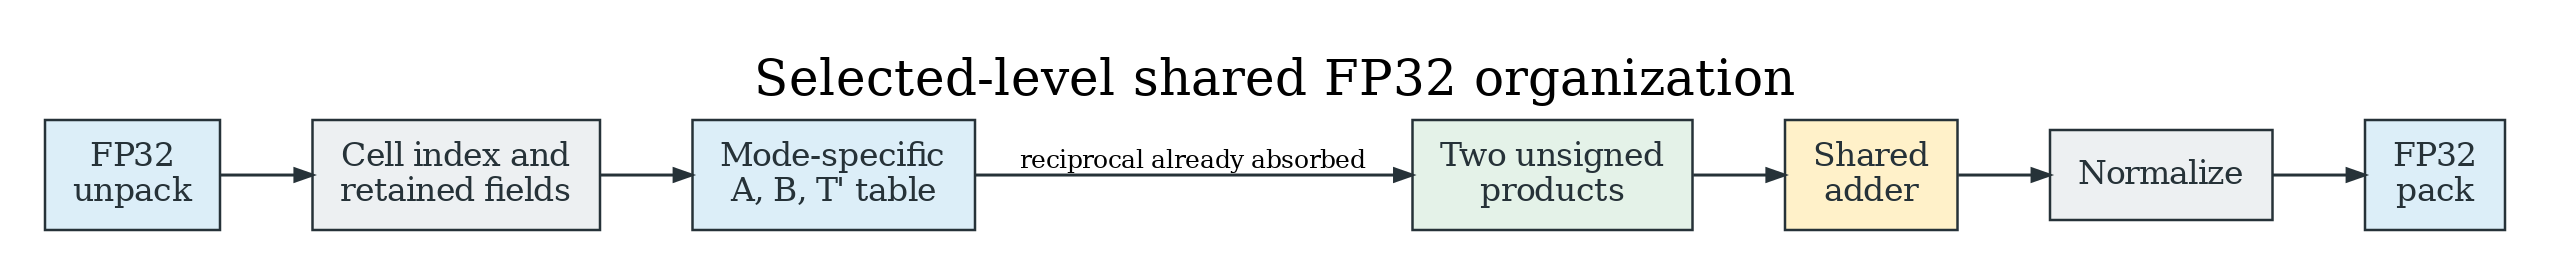
\includegraphics[width=0.96\textwidth]{pictures/structure.png}
\caption{Shared selected-level organization of the proposed STDM FP32
divider--multiplier. DIV and MUL select mode-specific coefficients for a
common two-product affine datapath.}
\label{fig:shared-arch}
\end{figure*}

For each implementation, the target level selects one local plane directly at
elaboration rather than retaining a chain of corrections from L0 to that level.
This distinction preserves the algebraic sharing between DIV and MUL without
requiring inter-level accumulation of an incremental
$\Delta z_i$/$\Delta w_i$ architecture.

The initial FP32 mantissa domain is $[1,2)\times[1,2)$. Level~0 uses this
whole domain as one cell. At level~1, each axis is split at $1.5$, producing
four rectangular subregions. In general, level~$n$ partitions each axis into
$2^n$ equal intervals:
\begin{equation}
 [x_{p-1}^n,x_p^n)\times[y_{q-1}^n,y_q^n),
\end{equation}
where $x_p^n=1+p/2^n$ and $y_q^n=1+q/2^n$ define the interval
boundaries along the $x$- and $y$-axes, respectively.
Fig.~\ref{fig:multilevel-partition} visualizes this recursive subdivision for
L0--L2; L3 continues the same bisection once more along each axis.

The midpoint of the selected cell is therefore
\begin{equation}
\begin{gathered}
 k_x^n=1+{2p(n)-1\over2^{n+1}},\\
 k_y^n=1+{2q(n)-1\over2^{n+1}}.
\end{gathered}
\end{equation}
where $p(n)$ and $q(n)$ are determined by the leading mantissa bits of $x$ and
$y$. Equivalently, starting from $k_x^0=k_y^0=3/2$, each deeper level updates
the midpoint by one signed binary step:
\begin{equation}
\begin{gathered}
 k_x^n=k_x^{n-1}+\sigma_x(n)2^{-(n+1)},\\
 k_y^n=k_y^{n-1}+\sigma_y(n)2^{-(n+1)}.
\end{gathered}
\label{eq:midpoint_update}
\end{equation}
where $\sigma_x(n),\sigma_y(n)\in\{-1,+1\}$ are selected by the $n$th
fractional bits.

These midpoint coordinates introduce no representation error. For L0--L3,
every midpoint is a dyadic rational with denominator at most 16 and is stored
exactly as the integer code $K=16k$. Thus midpoint selection and the products
used to form the untruncated local plane do not quantize $k_x^n$ or $k_y^n$.

Fig.~\ref{fig:selected-partition-point} shows that the same operand pair
$(x,y)$ lies in one cell at each partition level. As the level increases, the
grid becomes finer; the leading mantissa bits identify the finer cell that
contains $(x,y)$, and the center of that cell defines the level-dependent
midpoint $(k_x^n,k_y^n)$ used to evaluate the selected tangent plane.

\begin{figure*}[!b]
\centering
\begin{minipage}[t]{0.55\textwidth}
  \centering
  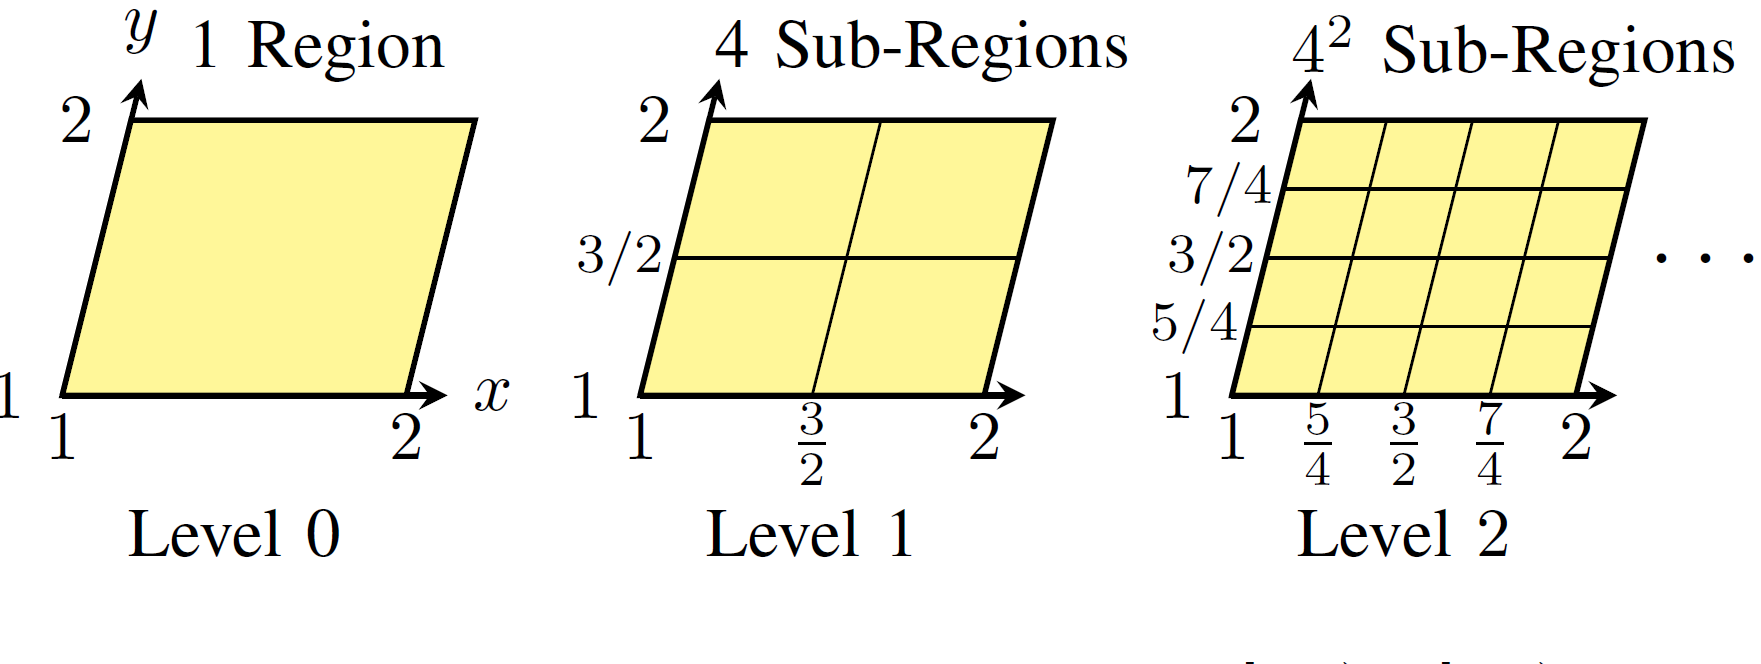
\includegraphics[width=\linewidth,trim=0 19pt 0 0,clip]
    {pictures/Figure 2.png}
  \captionof{figure}{Multi-level partition of the normalized mantissa domain.
  Each level bisects every interval along both axes.}
  \label{fig:multilevel-partition}
\end{minipage}
\hfill
\begin{minipage}[t]{0.38\textwidth}
  \centering
  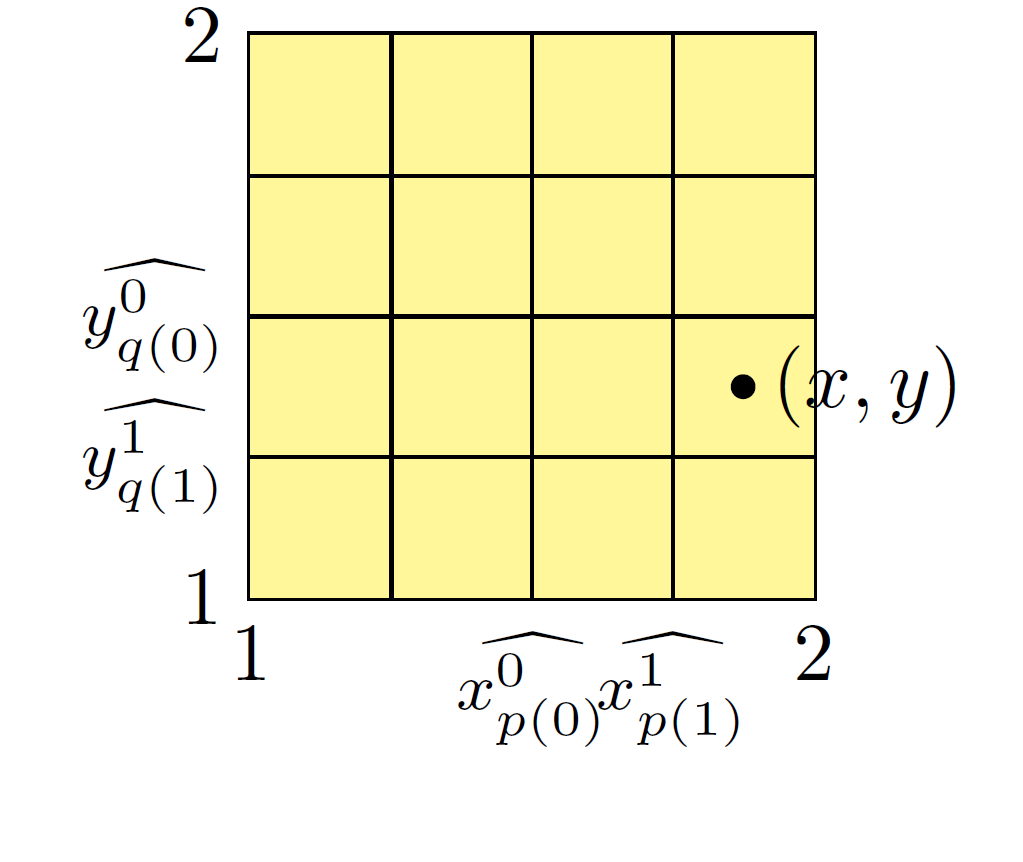
\includegraphics[width=0.86\linewidth,trim=0 20pt 0 0,clip]
    {pictures/Figure 3.png}
  \captionof{figure}{Selection of the local cell and midpoint coordinates for
  a mantissa pair $(x,y)$ in nested partitions.}
  \label{fig:selected-partition-point}
\end{minipage}
\end{figure*}

The remaining divider-specific factor is the reciprocal-square scale. Since
$k_y^n$ is fixed once the level and $y$-interval are known, the scale can be
precomputed and selected from a small table. For the L0--L3 levels used in this
work, the ideal constants are
\begin{align}
\text{L0:}\quad & {1\over(3/2)^2}, \nonumber\\
\text{L1:}\quad &
\begin{cases}
{1\over(5/4)^2}, & y[1]=0,\\
{1\over(7/4)^2}, & y[1]=1,
\end{cases} \nonumber\\
\text{L2:}\quad &
\begin{cases}
{1\over(9/8)^2},  & y[1:2]=00,\\
{1\over(11/8)^2}, & y[1:2]=01,\\
{1\over(13/8)^2}, & y[1:2]=10,\\
{1\over(15/8)^2}, & y[1:2]=11,
\end{cases} \nonumber\\
\text{L3:}\quad &
\begin{cases}
{1\over(17/16)^2}, & y[1:3]=000,\\
{1\over(19/16)^2}, & y[1:3]=001,\\
{1\over(21/16)^2}, & y[1:3]=010,\\
{1\over(23/16)^2}, & y[1:3]=011,\\
{1\over(25/16)^2}, & y[1:3]=100,\\
{1\over(27/16)^2}, & y[1:3]=101,\\
{1\over(29/16)^2}, & y[1:3]=110,\\
{1\over(31/16)^2}, & y[1:3]=111.
\end{cases}
\label{eq:recip_table}
\end{align}
Unlike the midpoints themselves, these reciprocal-square values generally do
not have finite binary representations. In particular, if
$k_y^n=K_y^n/16$, then $1/(k_y^n)^2=256/(K_y^n)^2$; after reduction, the
denominator normally retains an odd factor. For example, L0 requires
$1/(3/2)^2=4/9$, whose binary expansion repeats. As discussed in the next
section, STDM first quantizes and calibrates these values and then absorbs them
into the divider slopes and constant. The reciprocal code is therefore a
design parameter used to generate the table, not a separate multiplier operand
in the final RTL. This approximation does not alter the exact midpoint codes.

\iffalse
\section{Circuit Implementation and Optimization}
The original multi-level OAM hardware follows its recursive
derivation~\cite{chen2020oam}. Writing unscaled mantissa planes
generically as $P_n$, it first evaluates the L0 plane and then forms the
requested level as
\begin{equation}
    P_n = P_0 + \sum_{i=1}^{n}\Delta P_i .
    \label{eq:oam_level_recurrence}
\end{equation}
Here, $\Delta P_i$
updates the approximation from level $i-1$ to level $i$. Consequently, a
level-$n$ implementation contains
the L0 datapath, the correction generators $\Delta P_1,\ldots,\Delta P_n$, the
intermediate midpoint updates needed by those generators, and an accumulation
tree. This organization is useful when every successive approximation must be
available as an intermediate result, but that property is unnecessary in our
fixed-level STDM instances, where only the selected level plane is observed.

STDM therefore decodes the leading mantissa bits directly into the midpoint of
the selected level and evaluates that plane once. Before any bits are removed,
this selected-plane form is algebraically equivalent to evaluating
\eqref{eq:oam_level_recurrence} at the selected level; it changes the hardware
realization rather than the approximation algorithm. The direct plane is then
rewritten in coordinates relative to the center of each cell. This turns the two variable 24-bit mantissa products into products of a small
midpoint and a signed within-cell residual, and it exposes the same product
pair to DIV and MUL. The residuals themselves require no arithmetic
subtractor: because every midpoint lies at the center of a binary interval,
the exact subtraction is implemented by inverting the residual field's most
significant bit and sign-extending it.
An RTL miter over 200,000 randomized level/mode cases confirms that the direct
selected-level plane is bit-exact to the recurrence plane.

After these transformations, STDM applies least significant bit (LSB)
truncation at two points in the datapath. Residual truncation narrows
the signed operands entering the residual--midpoint multipliers. In DIV mode,
$w_n$ truncation additionally narrows the already combined plane operand
entering the reciprocal-coefficient multiplier. The reciprocal coefficients are then
calibrated against the packed FP32 output of each complete truncated datapath.
For MUL, which has no reciprocal stage, a midpoint-dependent bias
compensates the mean error introduced by residual truncation. Thus direct
level selection, centered residuals, and residual recoding are exact, whereas
the two LSB-truncation boundaries define the accuracy--PPA tradeoff.

\subsection{Centered-Residual Plane}
For the level-$n$ cell selected in the preceding derivation, define
\begin{equation}
 r_x^n=x-k_x^n,\qquad r_y^n=y-k_y^n.
 \label{eq:centered_residuals}
\end{equation}
Substituting $x=k_x^n+r_x^n$ and $y=k_y^n+r_y^n$ into
Eqs.~\eqref{eq:divplane} and~\eqref{eq:mulplane} gives
\begin{align}
 w_n &= k_x^nk_y^n+k_y^nr_x^n-k_x^nr_y^n,
 \label{eq:centered_div_plane}\\
 \widehat{m}_n &= k_x^nk_y^n+k_y^nr_x^n+k_x^nr_y^n.
 \label{eq:centered_mul_plane}
\end{align}
The divider and multiplier thus share the midpoint product and the same two
residual--midpoint products. Their unscaled planes differ only in the sign of
$k_x^nr_y^n$. Note that centering introduces no additional numerical error, because Eqs.~\eqref{eq:centered_div_plane}
and~\eqref{eq:centered_mul_plane} are exact rearrangements of the derived
tangent planes. Its hardware value is that $|r_x^n|$ and $|r_y^n|$ are bounded
by half a cell width and shrink as the partition level increases.

Let $m_x$ and $m_y$ denote the unsigned 24-bit Q23 mantissa integers. For
$n\in\{0,1,2,3\}$, the leading $n$ fraction bits directly form the local
interval indices
\begin{equation}
 \begin{aligned}
 i_x^n &=
 \begin{cases}
  0, & n=0,\\
  \lfloor(m_x-2^{23})/2^{23-n}\rfloor, & n>0,
 \end{cases}\\[4pt]
 i_y^n &=
 \begin{cases}
  0, & n=0,\\
  \lfloor(m_y-2^{23})/2^{23-n}\rfloor, & n>0.
 \end{cases}
 \end{aligned}
\end{equation}
Because every L0--L3 cell midpoint is an integer multiple of $1/16$, we use
a common denominator of 16 to avoid fractional midpoint arithmetic in the RTL. Let $K=16k$ denote the resulting exact integer midpoint code. Using
\begin{equation}
 B_n\in\{24,20,18,17\},\qquad S_n\in\{0,8,4,2\},
\end{equation}
for L0--L3, respectively, the selected midpoint numerators are
\begin{equation}
 K_x^n=B_n+S_ni_x^n,\qquad K_y^n=B_n+S_ni_y^n.
\end{equation}
As an example, for L3, $K=17+2i$, corresponding to
$17/16,19/16,\ldots,31/16$.

In the integer datapath, the exact Q23 residuals and centered divider plane are
\begin{align}
 R_x^n &=m_x-K_x^n2^{19},\qquad R_y^n=m_y-K_y^n2^{19},
 \label{eq:integer_residuals}\\
 W_n &=(K_x^nK_y^n)2^{15}+{K_y^nR_x^n\over16}
                         -{K_x^nR_y^n\over16}.
 \label{eq:integer_centered_plane}
\end{align}
A literal implementation of Eq.~\eqref{eq:integer_residuals} would use two
subtractors. Within a selected interval, however, midpoint subtraction is
merely the conversion of the lower residual field from offset binary to
two's complement. The hardware only inverts the local residual MSB and
sign-extends the remaining bits:
\begin{equation}
\begin{aligned}
 R_x^0 &= \{\,\overline{x_{22}},x_{21:0}\,\},\\
 R_x^1 &= \mathrm{sext}\{\,\overline{x_{21}},x_{20:0}\,\},\\
 R_x^2 &= \mathrm{sext}\{\,\overline{x_{20}},x_{19:0}\,\},\\
 R_x^3 &= \mathrm{sext}\{\,\overline{x_{19}},x_{18:0}\,\},
\end{aligned}
\label{eq:centered_residual_recode}
\end{equation}
and symmetrically for $R_y^n$. The natural signed residual widths
are consequently 23, 22, 21, and 20 bits for L0--L3. The exact centered plane
uses one pair of residual-by-midpoint products and one shared constant term:
\begin{gather}
 C_n = (K_x^nK_y^n)2^{15},\\
 T_x = (R_x^nK_y^n) \gg 4,\qquad
 T_y = (R_y^nK_x^n) \gg 4.
\end{gather}
Here, the arithmetic right shifts implement the factor $1/16$ from the midpoint encoding $k=K/16$.
For multiplication the plane is $C_n+T_x+T_y$, and for division it is
$C_n+T_x-T_y$ before reciprocal-square scaling. This similarity in the two planes, as we will discuss later, will result in significant area sharing.

\subsection{Residual and $w_n$ Truncation}
The centered formulation exposes two independent opportunities to remove
low-significance information. For a signed fixed-point integer $v$, define
\begin{equation}
 \mathcal{T}_D(v)=\left\lfloor{v\over2^D}\right\rfloor2^D.
 \label{eq:truncation_operator}
\end{equation}
, where $D$ is the number of truncated LSBs. The floor definition matters for negative two's-complement residuals: bit
slicing followed by zero padding rounds toward negative infinity, not toward
zero.

The first boundary is before the residual--midpoint products. When $D_r$
residual bits are truncated, Eq.~\eqref{eq:integer_centered_plane} becomes
\begin{equation}
 W'_n=(K_x^nK_y^n)2^{15}
 +{K_y^n\mathcal{T}_{D_r}(R_x^n)\over16}
 -{K_x^n\mathcal{T}_{D_r}(R_y^n)\over16}.
 \label{eq:residual_truncated_plane}
\end{equation}
Only the retained residual high bits enter the two multipliers; zero wiring
restores their original binary-point alignment. The common RTL container is
23-bit signed, but higher levels contain replicated sign-extension bits. The
independent retained information is therefore smaller than the declared slice
width at L1--L3.

The second truncation is only on DIV and occurs after the three terms in
Eq.~\eqref{eq:residual_truncated_plane} have been combined. We call it $w_n$ truncation because it removes low bits from the complete $kk+kr-kr$ plane,
rather than from either residual--midpoint product individually. The resulting
plane $W'_n$ is held in a 29-bit signed Q23 container, but for normal mantissas
it is nonnegative and below four, so only bits $[24:0]$ carry numerical
information. With $D_w$ low bits removed, the implemented divider mantissa is
\begin{equation}
 \begin{aligned}
 \widehat Z_n
 &=\underbrace{
 \left\lfloor{W'_n\over2^{D_w}}\right\rfloor 2^{D_w}
 }_{\text{truncated }W'_n}
 \cdot
 \underbrace{{C_{n,q}\over2^B}}_{\text{Q0.$B$ coefficient}}\\
 &=\left\lfloor{W'_n\over2^{D_w}}\right\rfloor
 C_{n,q}2^{D_w-B}.
 \end{aligned}
 \label{eq:wn_operand_truncation}
\end{equation}
where $q=i_y^n$ is the selected $y$-interval index, and $C_{n,q}/2^B$ is the
corresponding unsigned Q0.$B$ coefficient that approximates
$1/(k_y^n)^2$. The RTL stores the integer code $C_{n,q}$; division by $2^B$
specifies its fixed-point value and is realized by binary-point alignment, not
by a divider. Thus L0 stores the 7-bit integer $C_{0,0}=59$, which represents
the numerical coefficient $59/128$.

Table~\ref{tab:LSB-truncation} lists the selected divider DSE points
points for each level. ``Residual bits'' counts independent information after removing
redundant sign extension, and ``$w_n$ bits'' is the active plane width entering
the coefficient multiplier after $w_n$ truncation.

\begin{table*}[t]
\caption{Selected fixed-level divider precision and calibrated coefficient tables}
\label{tab:LSB-truncation}
\centering\scriptsize
\begin{tabular}{cccccccl}
\toprule
Level & $D_r$ & Residual bits & $D_w$ & $w_n$ bits & Format & Entries &
Coefficient integers in ascending $y$ intervals \\
\midrule
L0 & 18 & 5 & 18 & 7 & Q0.7 & 1 & $\{59\}$ \\
L1 & 16 & 6 & 16 & 9 & Q0.7 & 2 & $\{83,42\}$ \\
L2 & 16 & 5 & 16 & 9 & Q0.8 & 4 & $\{203,136,97,73\}$ \\
L3 & 16 & 4 & 16 & 9 & Q0.8 & 8 &
$\{227,182,149,124,105,90,78,68\}$ \\
\bottomrule
\end{tabular}
\end{table*}

Each fixed-level implementation propagates its target level at elaboration and
selects the residual precision, $w_n$ precision, and reciprocal-coefficient
format independently, as listed in Table~\ref{tab:LSB-truncation}.

\subsection{Error Compensation for MUL}
The same residual truncation applies to the multiplier plane, but it affects
the mean differently because both residual terms are added. We first derive
this effect in the normalized mantissa domain. Removing $D_r$ bits from a Q23
residual gives the truncation step
\[
 \Delta_r=2^{D_r-23},
\]
and the truncated residual is
\[
 \widetilde r=\Delta_r\left\lfloor{r\over\Delta_r}\right\rfloor.
\]
Define the discarded portions as
$\epsilon_x=r_x^n-\widetilde r_x^n$ and
$\epsilon_y=r_y^n-\widetilde r_y^n$. Assuming that the input mantissas are uniformly distributed within each partition, the discarded part of each residual is approximately uniform over $[0,\Delta_r)$, and hence
\[
 \mathrm{E}[\epsilon_x]\simeq\mathrm{E}[\epsilon_y]
 \simeq{\Delta_r\over2}=2^{D_r-24}.
\]
Let $\widetilde m_n$ denote the centered multiplier plane evaluated with
$\widetilde r_x^n$ and $\widetilde r_y^n$. Substituting
$\widetilde r=r-\epsilon$ into Eq.~\eqref{eq:centered_mul_plane} gives
\[
 \widetilde m_n-\widehat m_n
 =-k_y^n\epsilon_x-k_x^n\epsilon_y.
\]
Conditioned on the selected cell midpoints, the mean multiplier-plane error is
therefore
\[
 \mathrm{E}[\widetilde m_n-\widehat m_n]
 \simeq-(k_x^n+k_y^n)2^{D_r-24}.
\]
The corresponding compensation in the normalized mantissa domain is
$b_m=(k_x^n+k_y^n)2^{D_r-24}$. To obtain the integer added by the Q23 RTL, this
value is scaled by $2^{23}$. Using the exact midpoint encoding
$K_x^n=16k_x^n$ and $K_y^n=16k_y^n$ gives
\begin{equation}
 \begin{aligned}
 B_m
 &=2^{23}b_m\\
 &=(k_x^n+k_y^n)2^{D_r-1}\\
 &=(K_x^n+K_y^n)2^{D_r-5}.
 \end{aligned}
 \label{eq:mul_truncation_bias}
\end{equation}
This term uses the already available midpoint sum and a fixed shift to avoid
a multiplier correction table. The balanced multiplier points use
$D_r=16,14,12,10$ at L0--L3, retaining 7, 8, 9, 10 independent
residual bits, respectively.

Since the MUL datapath supplies the wider residual operands, the shared residual-midpoint multipliers are sized for the MUL operand width.
In DIV mode,
the more aggressively truncated residual high bits are followed by low zeros to
match this physical width; while in MUL mode, the wider retained residual is used
directly. A mode-controlled add/subtract selects $-T_y$ for division or
$+T_y+B_m$ for multiplication. Fig.~\ref{fig:circuit-structure} shows the detailed circuit structure of L0 STDM, where midpoint/index generation, both products, the
constant term, the plane adder, normalizer, FP32 wrapper, and output datapath
are shared. The reciprocal coefficient LUT and coefficient multiplier remain
divider-only, because multiplication has no corresponding operation.

\begin{figure*}[t]
\centering
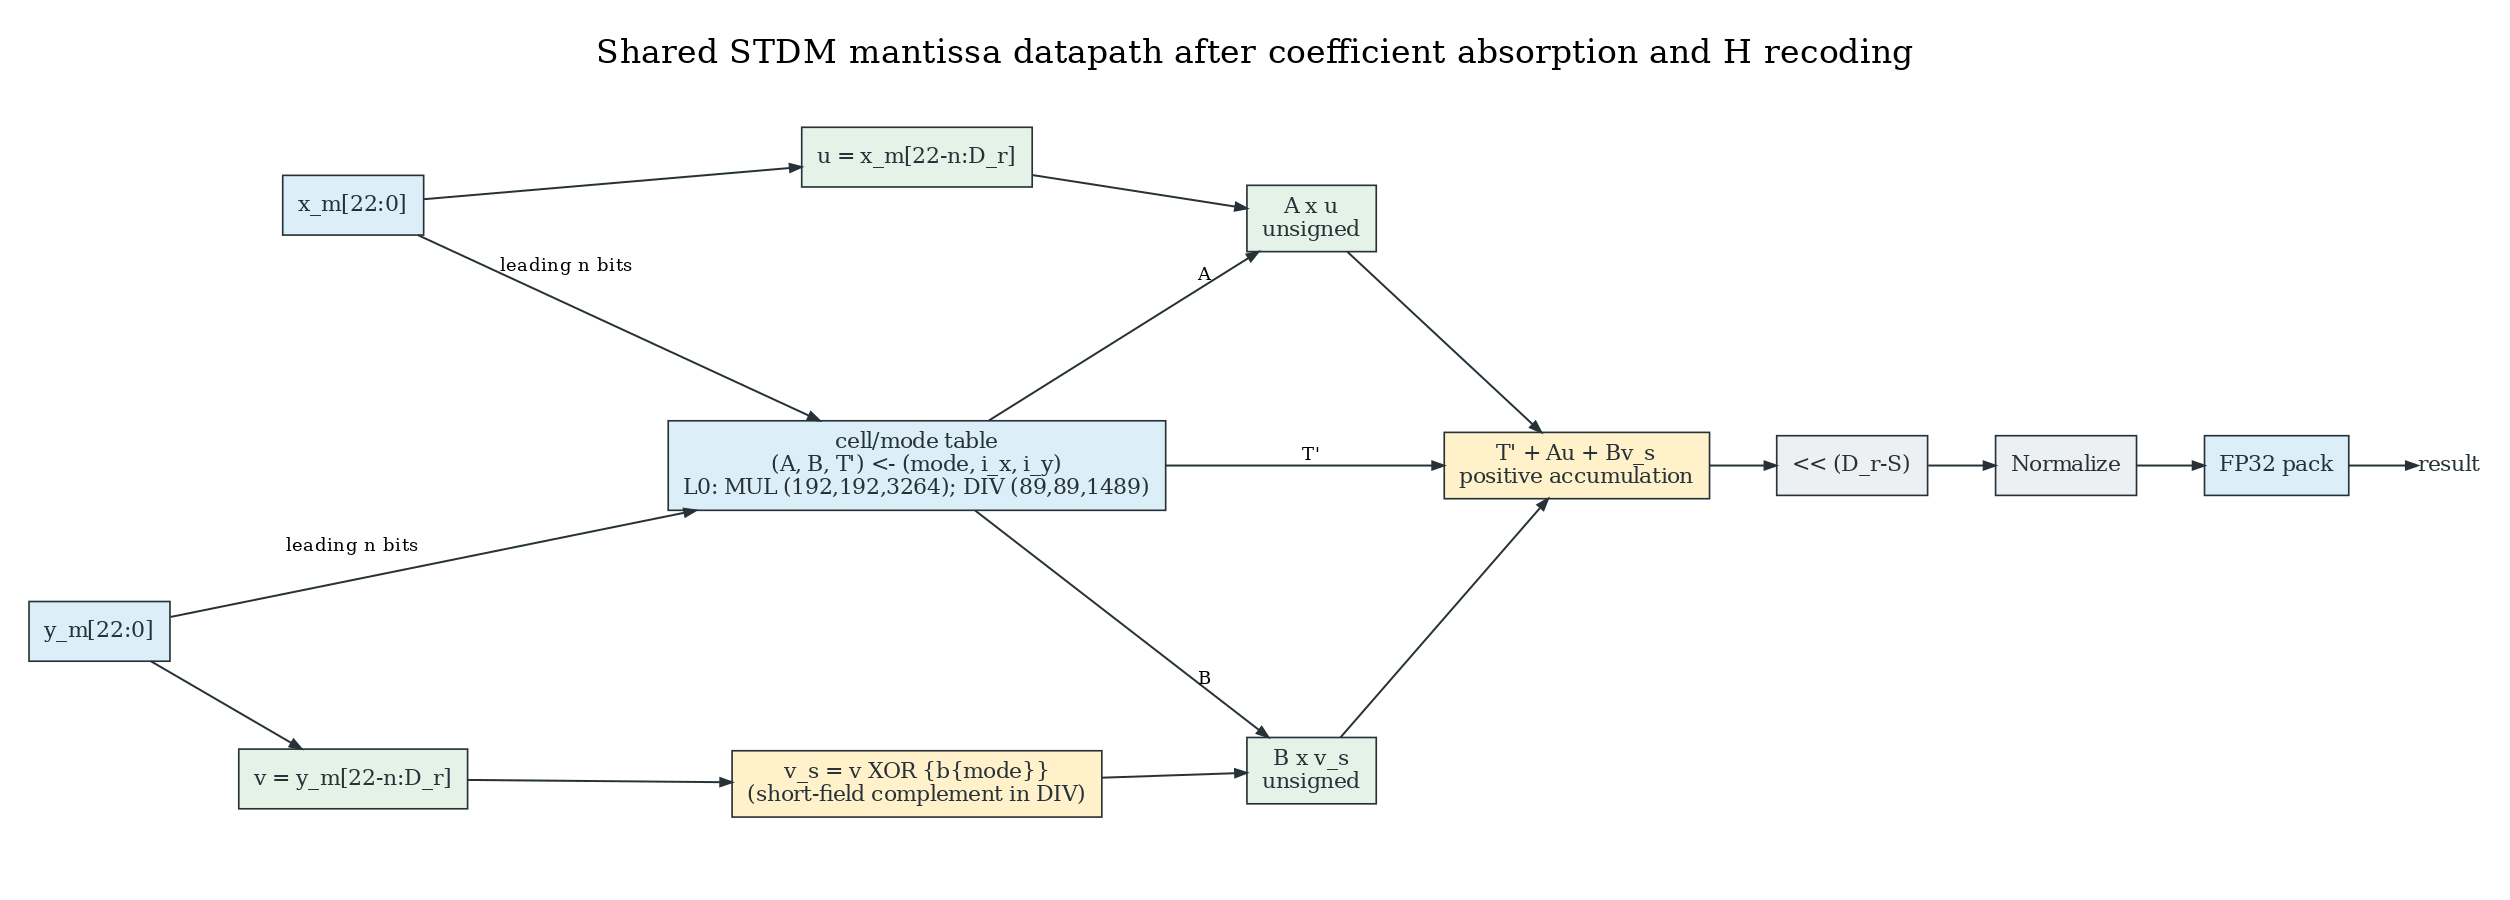
\includegraphics[width=0.96\textwidth]{pictures/circuit.png}
\caption{Circuit structure of the shared STDM FP32 divider--multiplier.}
\label{fig:circuit-structure}
\end{figure*}


\fi

\section{Circuit Implementation and Optimization}
The OAM derivation can be implemented recursively by evaluating L0 and adding
one correction for every deeper level. STDM instead fixes the target level at
elaboration, decodes the leading mantissa bits into the selected cell, and
evaluates that cell's affine function once. Before precision reduction, direct
selection is algebraically equivalent to
\begin{equation}
 P_n=P_0+\sum_{i=1}^{n}\Delta P_i,
 \label{eq:oam_level_recurrence}
\end{equation}
but it avoids the intermediate midpoint updates, correction generators, and
accumulation tree when only level $n$ is observable.

\subsection{Centered Residuals and Coefficient Absorption}
For the selected cell, define
\begin{equation}
 r_x^n=x-k_x^n,\qquad r_y^n=y-k_y^n.
 \label{eq:centered_residuals}
\end{equation}
Substitution into the two planes gives
\begin{align}
 \widehat m_n&=k_x^nk_y^n+k_y^nr_x^n+k_x^nr_y^n,
 \label{eq:centered_mul_plane}\\
 \widehat d_n&=c_n\left(k_x^nk_y^n+k_y^nr_x^n-k_x^nr_y^n\right),
 \quad c_n={1\over(k_y^n)^2}.
 \label{eq:centered_div_plane}
\end{align}
Centering is exact and bounds each residual by half the cell width. The leading
$n$ fraction bits select $k_x^n$ and $k_y^n$; the midpoint coordinates remain
the exact dyadic values derived in Section~III.

Let $R_x^n$ and $R_y^n$ be the Q23 integer residuals. After dropping $D_r$
low bits, the retained signed integers are
\begin{equation}
 \rho_x=\left\lfloor{R_x^n\over2^{D_r}}\right\rfloor,\qquad
 \rho_y=\left\lfloor{R_y^n\over2^{D_r}}\right\rfloor.
 \label{eq:retained_residuals}
\end{equation}
The residual width is only $b=23-n-D_r$ bits. Rather than first constructing
the unscaled divider plane and then multiplying it by $c_n$, STDM folds the
reciprocal factor into the cell coefficients. With $S$ fractional bits for the
slopes and $F=S+23-D_r$ fractional bits for the constant, the signed forms are
\begin{align}
 Q_M&=T_M+A_M\rho_x+B_M\rho_y,\label{eq:signed_mul_affine}\\
 Q_D&=T_D+A_D\rho_x-B_D\rho_y,\label{eq:signed_div_affine}
\end{align}
where
\begin{align}
 A_M&=\operatorname{round}(k_y^n2^S),&
 B_M&=\operatorname{round}(k_x^n2^S),\nonumber\\
 A_D&=\operatorname{round}(\bar c_nk_y^n2^S),&
 B_D&=\operatorname{round}(\bar c_nk_x^n2^S),
 \label{eq:absorbed_slopes}\\
 T_M&=\operatorname{round}((k_x^nk_y^n+b_M)2^F),&
 T_D&=\operatorname{round}(\bar c_nk_x^nk_y^n2^F).\nonumber
\end{align}
Here, $b_M$ is the residual-truncation bias derived below, and $\bar c_n$ is
the calibrated reciprocal-square coefficient. The represented mantissa value
is $Q2^{-F}$; equivalently, the RTL left shifts the integer sum by $D_r-S$ to
restore Q23 alignment. Equation~\eqref{eq:absorbed_slopes} is evaluated when
the tables are generated. Consequently, no reciprocal multiplication remains
in the synthesized datapath.

For multiplication, truncating a Q23 residual has step
$\Delta_r=2^{D_r-23}$. If the discarded portions are approximately uniform in
a cell, each has mean $\Delta_r/2$, giving the mantissa-domain correction
\begin{equation}
 b_M=(k_x^n+k_y^n)2^{D_r-24}.
 \label{eq:mul_truncation_bias}
\end{equation}
This correction is included in $T_M$ and therefore adds no hardware.

\subsection{Exact Unsigned Residual Recoding}
Equations~\eqref{eq:signed_mul_affine} and
\eqref{eq:signed_div_affine} still imply signed products and, for DIV, a
post-product subtraction. STDM removes both without changing the integer
result. Let $H=2^{b-1}$ and define the unsigned $b$-bit fields
\begin{equation}
 u=\rho_x+H,\qquad v=\rho_y+H.
 \label{eq:unsigned_residuals}
\end{equation}
Because the midpoint is the center of a binary interval, $u$ and $v$ are
exactly the retained local mantissa fields; no subtractor is required. For MUL,
\begin{equation}
 Q_M=\underbrace{T_M-H(A_M+B_M)}_{T'_M}+A_Mu+B_Mv.
 \label{eq:unsigned_mul_affine}
\end{equation}
For DIV, let $\bar v=(2H-1)-v$, which is the bitwise complement of the $b$-bit
field $v$. Then
\begin{equation}
 Q_D=\underbrace{T_D-H(A_D+B_D)+B_D}_{T'_D}
       +A_Du+B_D\bar v.
 \label{eq:unsigned_div_affine}
\end{equation}
Thus operation control only selects the mode-specific table entry and either
$v$ or its short bitwise complement. Both products are unsigned and the main
adder only accumulates nonnegative terms. The changes from $T$ to $T'$ are
performed offline when the coefficient table is generated. Exhaustive checks
over every retained residual code and every table entry, followed by RTL and
gate-level regression, confirmed word-identical outputs to the signed forms.

Table~\ref{tab:implementation_precision} lists the shared-unit precisions. All
mode-specific values of $A$, $B$, and $T'$ are selected by the operation bit
and the leading mantissa bits. Within each level, DIV and MUL use the same
coefficient precision; in particular, the L1 shared unit uses the same $S=4$
precision as the selected DIV-only L1 implementation.

\begin{table}[t]
\caption{Precision of the shared STDM mantissa datapath}
\label{tab:implementation_precision}
\centering\small
\begin{tabular}{ccccc}
\toprule
Level & $D_r$ & $b$ & $S$ & $F=S+23-D_r$ \\
\midrule
L0 & 18 & 5 & 6 & 11 \\
L1 & 16 & 6 & 4 & 11 \\
L2 & 16 & 5 & 5 & 12 \\
L3 & 16 & 4 & 4 & 11 \\
\bottomrule
\end{tabular}
\end{table}

Fig.~\ref{fig:circuit-structure} shows the resulting organization. Cell and
mode bits address a compact table containing the already absorbed and recoded
$A$, $B$, and $T'$ values. The retained $x$ field feeds one unsigned product;
the retained $y$ field is complemented only in DIV mode and feeds the other.
Their outputs and $T'$ enter a common adder, followed by fixed binary-point
alignment, normalization, exponent handling, and FP32 packing. There is no
level-correction chain, signed residual multiplier, wide conditional
subtractor, or post-plane reciprocal multiplier.

\begin{figure*}[t]
\centering
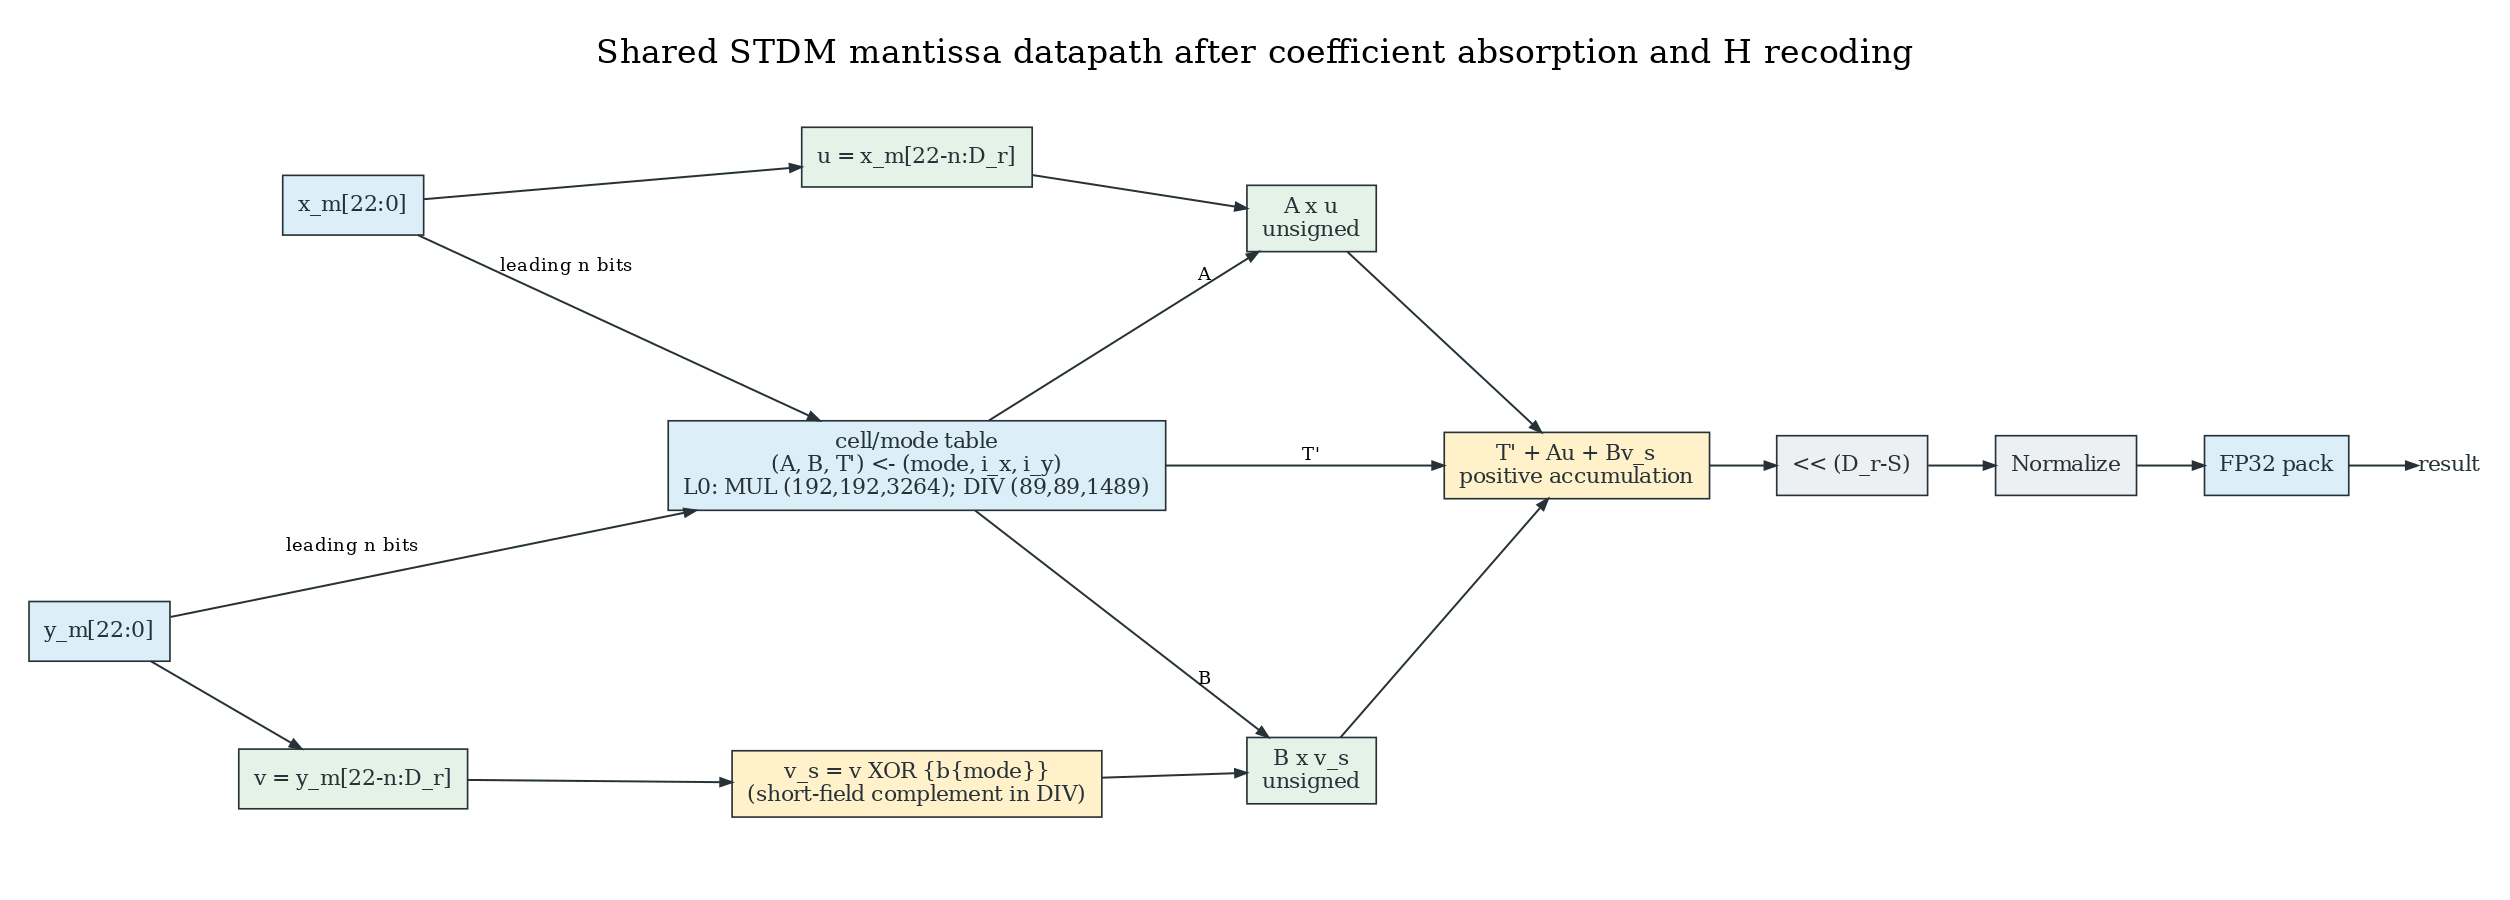
\includegraphics[width=0.96\textwidth]{pictures/circuit.png}
\caption{Circuit structure of the shared STDM FP32 divider--multiplier after
coefficient absorption and exact unsigned residual recoding.}
\label{fig:circuit-structure}
\end{figure*}

\section{Evaluation and Discussion}
\subsection{Evaluation Protocol}
\label{sec:evaluation-protocol}
All reported PPA uses Design Compiler U-2022.12-SP7 and PrimeTime
U-2022.12-SP5 with the TSMC 65-nm typical CCS library. The designs are
combinational, with no clock port or sequential area. The 10-ns virtual clock
has zero uncertainty, 20-ps input/output delays, an \texttt{INVD0} input
driver, and 0.004 output load. PT reads the synthesized netlist and SDC,
checks timing, and applies static probability 0.5 and toggle rate 0.1 per
10-ns period to all inputs. PDP is the product of delay and power and is
reported in fJ; ADP is the product of area and delay.

All approximate operators have 32-bit FP32 inputs and outputs and are evaluated
on normal finite operands. A common wrapper extracts the two 24-bit normalized
mantissas, computes the result sign and exponent, applies the normalization
shift reported by the mantissa core, and packs the FP32 output. The wrapper is
included in every reported PPA result. Subnormal numbers, infinities, NaNs, and
exponent overflow or underflow are outside the present evaluation scope.

The DIV-only evaluation includes the four H-recoded STDM specializations,
author-provided PACE mantissa RTL, and local reconstructions of PLSAD and FPD2D.
PACE is connected to its normal-FP32 wrapper without changing its mantissa
arithmetic. PLSAD reconstructs the paper's ten-bit, eight-plane configuration
with an eight-bit exact upper adder. FPD2D reconstructs its $8\times8$ fused
linear architecture; because the printed coefficient table contains anomalous
cells, the three reported rows use an independent implementation of the
paper's coefficient-optimization algorithm rather than silently modifying the
printed table. These reconstructions are not presented as author RTL. STDM,
PACE, PLSAD, and FPD2D are evaluated on the same 200,000 positive normalized
FP32 operand pairs and complete packed outputs. FaNZeD, TruncApp, LEAD, and
QIAD remain as broader local implementation context; their arithmetic and
previously documented accuracy sets are unchanged. LEAD's supplied two phases
are combinationally unrolled and verified against the original two-phase RTL.

The complete DIV+MUL evaluation uses one external reference. The exact reference
instantiates DesignWare \texttt{DW\_fp\_div} and \texttt{DW\_fp\_mult} in
parallel and selects their outputs with the same operation control exposed by
STDM. Both DesignWare operators are combinational FP32 blocks and are included
in full, so this reference contains no arithmetic sharing between division and
multiplication. It is a cost reference for exact FP32 support, not an
accuracy-matched competitor. No prior approximate combined unit is placed in
the table: SIMDive has an integer SIMD FPGA interface, while the other fused
units reviewed in Section~II compute exact results with different timing
contracts.

\begin{table*}[!t]
\caption{DIV-only accuracy and hardware results. STDM, PACE, PLSAD, and FPD2D
use the same 200,000-input accuracy set.}
\label{tab:div_comparison}
\centering\scriptsize
\setlength{\tabcolsep}{2.4pt}
\begin{tabular}{lrrrrrrrr}
\toprule
Design & MAE & MRED & RMSE & Area (\um) & Delay (ns) & Power (mW) & PDP (fJ) & Norm. ADP \\
\midrule
Exact DesignWare DIV & -- & -- & -- & 19604.52 & 9.750 & 1.89509 & 18477.43 & 1.0000 \\
\midrule
STDM L0 & 0.042818 & 0.042856 & 0.056227 & 525.60 & 1.401 & 0.02103 & 29.47 & 0.0039 \\
STDM L1 & 0.011796 & 0.011263 & 0.016233 & 809.64 & 1.685 & 0.03132 & 52.78 & 0.0071 \\
STDM L2 & 0.003778 & 0.003568 & 0.005105 & 1030.32 & 1.940 & 0.03094 & 60.03 & 0.0105 \\
STDM L3 & 0.002663 & 0.002577 & 0.003430 & 1149.12 & 2.006 & 0.03004 & 60.26 & 0.0121 \\
\midrule
PACE L1 & 0.028163 & 0.025951 & 0.045176 & 990.00 & 2.214 & 0.04467 & 98.92 & 0.0115 \\
PACE L2 & 0.015143 & 0.014859 & 0.022305 & 1551.60 & 2.362 & 0.07829 & 184.88 & 0.0192 \\
PACE L3 & 0.005897 & 0.005608 & 0.009281 & 2271.96 & 2.821 & 0.13119 & 370.08 & 0.0335 \\
PACE L4 & 0.003856 & 0.003816 & 0.006060 & 3150.72 & 2.987 & 0.18531 & 553.51 & 0.0492 \\
\midrule
PLSAD ($m=8$) & 0.008975 & 0.008709 & 0.013227 & 659.88 & 1.738 & 0.02414 & 41.96 & 0.0060 \\
FPD2D $8\times8,t=17$ & 0.005344 & 0.005282 & 0.006828 & 790.56 & 1.873 & 0.01981 & 37.09 & 0.0077 \\
FPD2D $8\times8,t=16$ & 0.004054 & 0.004096 & 0.005134 & 869.76 & 1.962 & 0.02328 & 45.67 & 0.0089 \\
FPD2D $8\times8,t=15$ & 0.003653 & 0.003735 & 0.004636 & 942.12 & 2.038 & 0.02660 & 54.22 & 0.0100 \\
\midrule
FaNZeD & 0.031811 & 0.031130 & 0.046191 & 2775.96 & 4.968 & 0.08880 & 441.16 & 0.0721 \\
TruncApp & 0.120105 & 0.119617 & 0.162391 & 4581.36 & 3.133 & 0.26136 & 818.77 & 0.0751 \\
LEAD & 0.021750 & 0.020993 & 0.028841 & 6666.12 & 5.674 & 0.60630 & 3440.38 & 0.1979 \\
QIAD & 0.005889 & 0.005880 & 0.006940 & 12097.80 & 8.074 & 0.95201 & 7686.66 & 0.5110 \\
\bottomrule
\end{tabular}
\end{table*}

\begin{table*}[!b]
\caption{Accuracy and hardware results for designs supporting both DIV and MUL.}
\label{tab:divmul_comparison}
\centering\scriptsize
\setlength{\tabcolsep}{3.2pt}
\begin{tabular}{lrrrrrrr}
\toprule
Design & DIV MRED & MUL MRED & Area (\um) & Delay (ns) & Power (mW) & PDP (fJ) & ADP ($\mu\mathrm{m}^2\mathrm{ns}$) \\
\midrule
Exact DesignWare DIV+MUL & -- & -- & 24025.68 & 9.856 & 2.08421 & 20541.66 & 236793.50 \\
\midrule
STDM L0 & 0.042856 & 0.032453 & 891.36 & 1.836 & 0.03415 & 62.71 & 1636.94 \\
STDM L1 & 0.011263 & 0.007903 & 1183.32 & 2.136 & 0.03932 & 83.99 & 2527.95 \\
STDM L2 & 0.003568 & 0.002687 & 1454.40 & 2.401 & 0.03797 & 91.17 & 3492.15 \\
STDM L3 & 0.002577 & 0.001901 & 1794.96 & 2.509 & 0.03944 & 98.95 & 4503.29 \\
\bottomrule
\end{tabular}
\end{table*}

\iffalse
\subsection{Theoretical Error Analysis}
We first consider the local divider plane before residual truncation,
$w_n$ truncation, and reciprocal coefficient encoding. Let
$f(x,y)=x/y$, and let $(k_x^n,k_y^n)$ be the midpoint of the level-$n$ cell
containing $(x,y)$. For some $0<\theta<1$, Taylor's theorem gives
\begin{equation}
\begin{aligned}
f(x,y)={}&f(k_x^n,k_y^n)\\
&+r_x^n f_x(k_x^n,k_y^n)
 +r_y^n f_y(k_x^n,k_y^n)\\
&+\frac{1}{2}(r_x^n)^2f_{xx}(\xi_x,\xi_y)\\
&+r_x^nr_y^nf_{xy}(\xi_x,\xi_y)\\
&+\frac{1}{2}(r_y^n)^2f_{yy}(\xi_x,\xi_y),
\end{aligned}
\label{eq:taylor_remainder}
\end{equation}
where
\begin{equation}
 \xi_x=k_x^n+\theta r_x^n,\qquad
 \xi_y=k_y^n+\theta r_y^n.
\end{equation}
The first three terms in Eq.~\eqref{eq:taylor_remainder} are exactly the
divider plane $\widehat d_n$ derived in Section~III. Since
$f_{xx}=0$, $f_{xy}=-1/y^2$, and $f_{yy}=2x/y^3$, the remaining error is
\begin{equation}
\begin{aligned}
e_n
&=\frac{x}{y}-\widehat d_n\\
&=-\frac{r_x^nr_y^n}{\xi_y^2}
  +\frac{(r_y^n)^2\xi_x}{\xi_y^3}\\
&=\frac{r_y^n(r_y^n\xi_x-r_x^n\xi_y)}{\xi_y^3}.
\end{aligned}
\label{eq:divider_remainder}
\end{equation}

Each level-$n$ interval has width $2^{-n}$, so midpoint selection guarantees
$|r_x^n|,|r_y^n|\leq2^{-(n+1)}$. Moreover,
$1\leq\xi_y<2$ and $1\leq\xi_x<2$ for normalized mantissas. It follows that
\begin{equation}
\begin{aligned}
|e_n|
&\leq |r_y^n|\left(2|r_y^n|+2|r_x^n|\right)\\
&\leq \frac{1}{2^{n+1}}\frac{4}{2^{n+1}}
=\frac{1}{4^n}.
\end{aligned}
\label{eq:divider_error_bound}
\end{equation}
Thus each additional partition level reduces this worst case bound by a factor
of four. The bound characterizes the piecewise tangent approximation itself.

We next include the two truncation operations used by the divider. Removing
$D_r$ bits from a Q23 residual gives the step
$\Delta_r=2^{D_r-23}$. Write the truncated residuals as
$\widetilde r_x^n=r_x^n-\epsilon_x$ and
$\widetilde r_y^n=r_y^n-\epsilon_y$, where
$0\leq\epsilon_x,\epsilon_y<\Delta_r$. Substitution into
Eq.~\eqref{eq:centered_div_plane} gives the plane after residual truncation:
\begin{equation}
 w_n^{(r)}=w_n-k_y^n\epsilon_x+k_x^n\epsilon_y.
 \label{eq:divider_residual_truncation_error}
\end{equation}
The opposite signs are important: the errors from the two truncated residuals
can partially cancel rather than always accumulate.

The Q23 plane is then truncated with step
$\Delta_w=2^{D_w-23}$. Define
\begin{equation}
 \epsilon_w=w_n^{(r)}-
 \Delta_w\left\lfloor{w_n^{(r)}\over\Delta_w}\right\rfloor,
 \qquad 0\leq\epsilon_w<\Delta_w,
\end{equation}
so that the plane entering the reciprocal coefficient multiplier is
$\widetilde w_n=w_n^{(r)}-\epsilon_w$. If the exact coefficient
$c_n=1/(k_y^n)^2$ is used, the divider error after both truncations is
\begin{equation}
\begin{aligned}
 e_n^{(t)}
 &= {x\over y}-c_n\widetilde w_n\\
 &=e_n+{k_y^n\epsilon_x-k_x^n\epsilon_y+\epsilon_w
          \over(k_y^n)^2}.
\end{aligned}
\label{eq:divider_total_truncation_error}
\end{equation}
Therefore, the additional absolute error caused by truncation satisfies
\begin{equation}
\begin{aligned}
 \left|e_n^{(t)}-e_n\right|
 &<{(k_x^n+k_y^n)\Delta_r+\Delta_w\over(k_y^n)^2}\\
 &\leq 4\Delta_r+\Delta_w,\\
 \left|e_n^{(t)}\right|
 &<{1\over4^n}
   +{(k_x^n+k_y^n)\Delta_r+\Delta_w\over(k_y^n)^2}.
\end{aligned}
 \label{eq:divider_truncation_error_bound}
\end{equation}
The first inequality is cell dependent and is the more useful bound for a
selected level. The second follows from $1\leq k_x^n,k_y^n<2$ and provides a
simple bound over the complete normalized mantissa domain.

For intuition, if the discarded portions are approximately uniform within a
cell, their means are close to half of their respective truncation steps. The
mean additional error is then
\begin{equation}
\begin{aligned}
 &\mathrm{E}\!\left[e_n^{(t)}-e_n\mid k_x^n,k_y^n\right]\\
 &\qquad\simeq {(k_y^n-k_x^n)\Delta_r+\Delta_w
                 \over2(k_y^n)^2}.
\end{aligned}
 \label{eq:divider_mean_truncation_error}
\end{equation}
This expression also explains why the two truncation parameters cannot be
selected from operand width alone: residual truncation has a midpoint-dependent
signed contribution, whereas $w_n$ truncation always lowers the plane before
reciprocal scaling. Coefficient encoding adds a final term. If
$\bar c_n=C_{n,q}/2^B=c_n+\delta_c$, the complete mantissa error is
\begin{equation}
 e_n^{(\mathrm{hw})}=e_n^{(t)}-\delta_c\widetilde w_n.
 \label{eq:divider_complete_error}
\end{equation}
Normalization and FP32 packing are included in the measured errors reported
below. The next subsection explains how $\delta_c$ is selected for this
complete datapath.

\subsection{Reciprocal Coefficient Calibration}
The integer nearest to $2^B/(k_y^n)^2$ minimizes the error of the reciprocal
coefficient alone, but it does not always minimize the error of the complete divider.
Let $C_0=1/(k_y^n)^2$, let $\widetilde w_n$ denote the plane after residual and
$w_n$ truncation, and define $e_0=x/y-C_0\widetilde w_n$. Replacing $C_0$ by
$C_0+\delta$ gives
\begin{equation}
 \mathrm{E}[e^2]=\mathrm{E}[e_0^2]
 -2\delta\mathrm{E}[e_0\widetilde w_n]
 +\delta^2\mathrm{E}[\widetilde w_n^2].
 \label{eq:coefficient_calibration}
\end{equation}
The plane error and truncation error are correlated with $\widetilde w_n$.
Consequently, a neighboring coefficient can give a lower final MSE than the
integer nearest to the ideal reciprocal value.

Fig.~\ref{fig:l0-coefficient-sweep} shows this effect for L0. The ideal
coefficient is $1/(3/2)^2=4/9$, whose nearest Q0.7 representation is $57/128$.
For the selected $D_r=D_w=18$ datapath, $57/128$ gives an RMSE of 0.07119,
whereas $59/128$ gives the minimum RMSE of 0.05663 in the tested range.
The coefficient $58/128$ gives the lowest MAE and MRED, while $59/128$ is
selected because calibration uses MSE as its objective. The coefficients at
the other levels are selected in the same manner for their complete FP32
datapaths.

\begin{figure}[t]
\centering
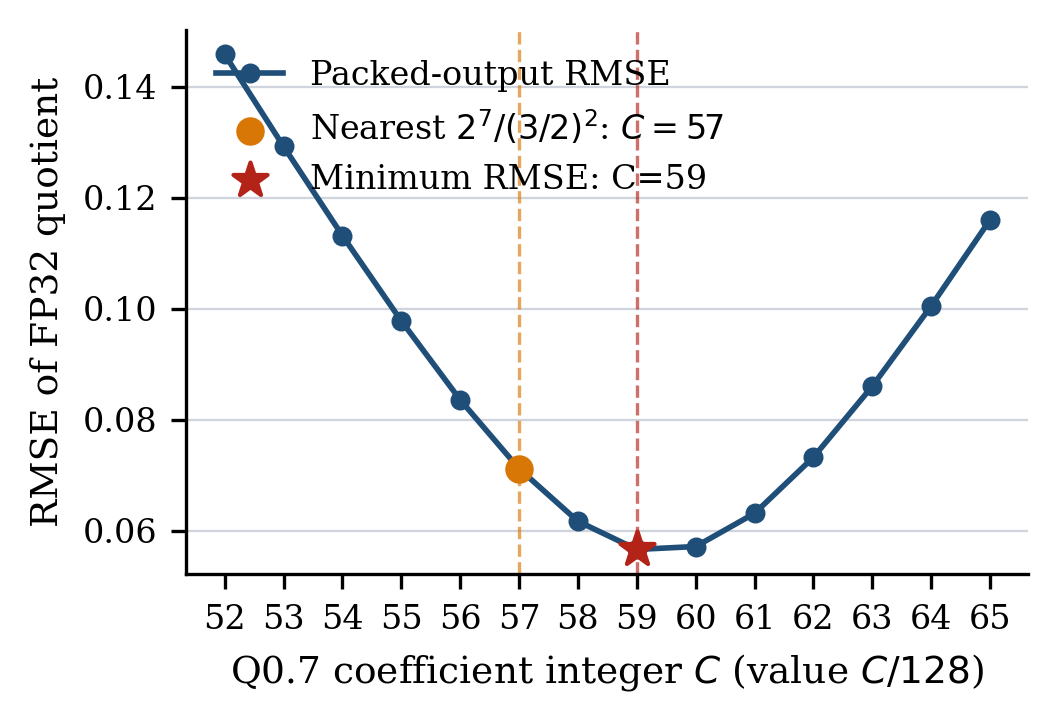
\includegraphics[width=\columnwidth]{pictures/l0_q07_coefficient_sweep.png}
\caption{L0 reciprocal coefficient calibration for the selected
$D_r=D_w=18$ datapath. The coefficient nearest to $4/9$ is $57/128$, while
$59/128$ minimizes the RMSE of the complete FP32 divider.}
\label{fig:l0-coefficient-sweep}
\end{figure}

\fi

\subsection{Theoretical Error Analysis}
Let $f(x,y)=x/y$ and let $(k_x^n,k_y^n)$ be the midpoint of the selected
level-$n$ cell. The first-order Taylor terms give
Eq.~\eqref{eq:centered_div_plane}. Since $f_{xx}=0$,
$f_{xy}=-1/y^2$, and $f_{yy}=2x/y^3$, the remainder can be written as
\begin{equation}
 e_n={x\over y}-\widehat d_n
 ={r_y^n(r_y^n\xi_x-r_x^n\xi_y)\over\xi_y^3},
 \label{eq:divider_remainder}
\end{equation}
where $\xi_x=k_x^n+\theta r_x^n$, $\xi_y=k_y^n+\theta r_y^n$, and
$0<\theta<1$. A level-$n$ cell has width $2^{-n}$, so
$|r_x^n|,|r_y^n|\leq2^{-(n+1)}$. With normalized mantissas,
\begin{equation}
 |e_n|\leq |r_y^n|(2|r_y^n|+2|r_x^n|)\leq4^{-n}.
 \label{eq:divider_error_bound}
\end{equation}
Thus partition refinement reduces the bound on the tangent approximation by a
factor of four per level.

Residual truncation introduces a separate error. Write
$\widetilde r_x^n=r_x^n-\epsilon_x$ and
$\widetilde r_y^n=r_y^n-\epsilon_y$, where
$0\leq\epsilon_x,\epsilon_y<\Delta_r=2^{D_r-23}$. Before coefficient
quantization, the divider error becomes
\begin{equation}
 e_n^{(r)}=e_n+c_n(k_y^n\epsilon_x-k_x^n\epsilon_y).
 \label{eq:divider_residual_truncation_error}
\end{equation}
The opposite signs allow partial cancellation. A simple cell-dependent bound is
\begin{equation}
 |e_n^{(r)}-e_n|<c_n(k_x^n+k_y^n)\Delta_r.
 \label{eq:divider_truncation_error_bound}
\end{equation}

Finally, let $A_D^*$, $B_D^*$, and $T_D^*$ denote the ideally scaled
coefficients in Eq.~\eqref{eq:absorbed_slopes}, and define their integer
quantization errors as $\delta_A=A_D-A_D^*$,
$\delta_B=B_D-B_D^*$, and $\delta_T=T_D-T_D^*$. Coefficient absorption adds
\begin{equation}
 e_n^{(q)}-e_n^{(r)}
 =2^{-F}(\delta_T+\delta_A\rho_x-\delta_B\rho_y).
 \label{eq:absorbed_quantization_error}
\end{equation}
This term depends on both the cell and retained residuals, so choosing a base
reciprocal solely by its distance from $1/(k_y^n)^2$ need not minimize the
error of the implemented FP32 divider. The unsigned recoding in
Eqs.~\eqref{eq:unsigned_mul_affine} and
\eqref{eq:unsigned_div_affine} is an integer identity and adds no error.

\subsection{Reciprocal Coefficient Calibration}
For each $y$ interval, neighboring fixed-point reciprocal codes are evaluated
through residual truncation, absorbed coefficient generation, normalization,
and FP32 packing. If $C_0=1/(k_y^n)^2$, $w$ denotes the corresponding
truncated plane, and $e_0=x/y-C_0w$, replacing $C_0$ by $C_0+\delta$ changes
the mean squared error according to
\begin{equation}
 \mathrm{E}[e^2]=\mathrm{E}[e_0^2]
 -2\delta\mathrm{E}[e_0w]+\delta^2\mathrm{E}[w^2].
 \label{eq:coefficient_calibration}
\end{equation}
Because plane error and coefficient error are correlated, the nearest code is
not necessarily the best end-to-end code. For example, the ideal L0 value is
$4/9$ and its nearest Q0.7 code is $57/128$, but the complete calibration
sweep selects $59/128$ for minimum RMSE. This code is subsequently folded into
$A_D$, $B_D$, and $T_D$; $59$ is not a standalone multiplier operand in the
final circuit.

\begin{figure}[t]
\centering
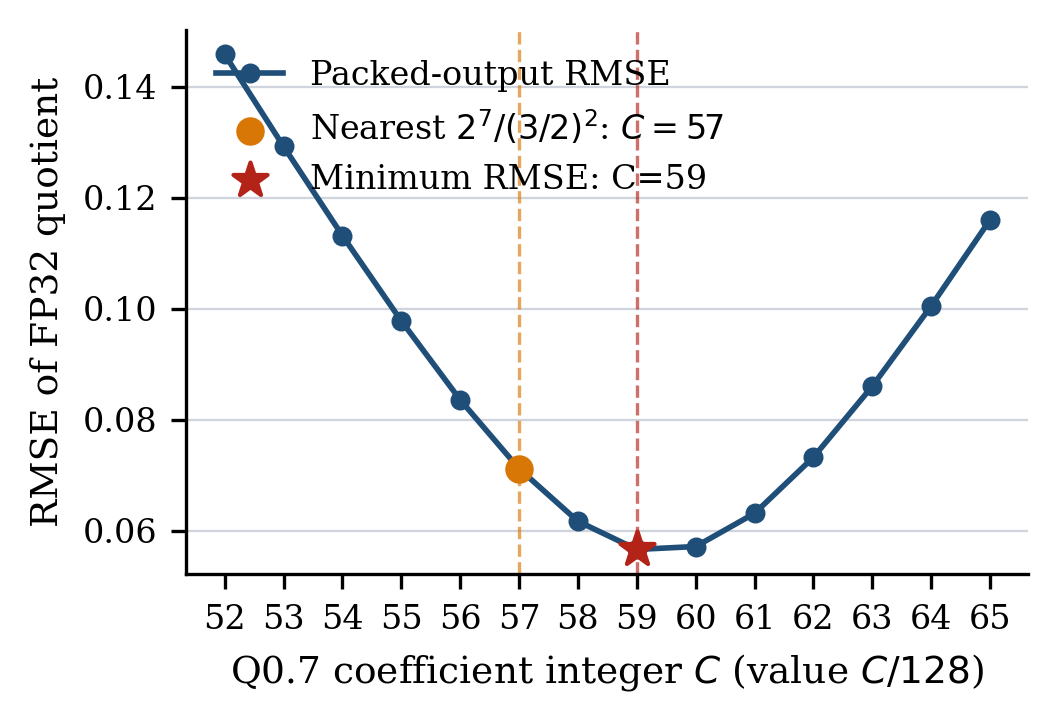
\includegraphics[width=\columnwidth]{pictures/l0_q07_coefficient_sweep.png}
\caption{L0 end-to-end reciprocal-code calibration. The code nearest to
$4/9$ is 57, whereas code 59 minimizes the complete-divider RMSE before
coefficient absorption.}
\label{fig:l0-coefficient-sweep}
\end{figure}

\subsection{DIV-Only Comparison}
Table~\ref{tab:div_comparison} compares the four STDM dividers with PACE and
the locally implemented prior dividers. All hardware results use the common
FP32 interface and synthesis conditions described in
Section~\ref{sec:evaluation-protocol}. The ADP values are normalized to the
exact DesignWare divider. These rows are DIV-only specializations, whereas
Table~\ref{tab:divmul_comparison} reports the complete shared units.

STDM L1--L3 have lower MAE, MRED, and RMSE than PACE L2--L4, respectively,
while using less area, delay, and power in every paired comparison. PLSAD is
smaller than STDM L1 but lies between STDM L1 and L2 in all three error
measures. The reconstructed FPD2D points define a strong low-cost region:
$8\times8,t=16$ nearly matches STDM L2, while $t=15$ trades lower RMSE for
higher MRED. STDM L3 is more accurate than all three evaluated FPD2D points,
but requires more area and power than $t=15$. Thus STDM does not claim the best
isolated divider at every error target; its additional value is a divider plane
that can share its dominant arithmetic with multiplication. STDM L3 uses
94.1\% less area, 79.4\% less delay, and 98.4\% less power than the exact
divider, with a normalized ADP of 0.0121.

\begin{table}[!t]
\caption{Effect of sharing arithmetic between DIV and MUL. Percentages in
Shared rows are changes relative to Separate at the same level.}
\label{tab:sharing_comparison}
\centering\scriptsize
\resizebox{\columnwidth}{!}{%
\begin{tabular}{clrrrrr}
\toprule
Level & Structure & Area (\um) & Delay (ns) & Power (mW) & PDP (fJ) & ADP ($\mu\mathrm{m}^2\mathrm{ns}$) \\
\midrule
L0 & Separate & 911.88 & 1.649 & 0.03451 & 56.89 & 1503.44 \\
   & Shared & \shortstack{891.36\\(-2.3\%)} & \shortstack{1.836\\(+11.3\%)} & \shortstack{0.03415\\(-1.0\%)} & \shortstack{62.71\\(+10.2\%)} & \shortstack{1636.94\\(+8.9\%)} \\
L1 & Separate & 1429.20 & 2.005 & 0.05746 & 115.23 & 2866.09 \\
   & Shared & \shortstack{1183.32\\(-17.2\%)} & \shortstack{2.136\\(+6.5\%)} & \shortstack{0.03932\\(-31.6\%)} & \shortstack{83.99\\(-27.1\%)} & \shortstack{2527.95\\(-11.8\%)} \\
L2 & Separate & 1796.40 & 2.271 & 0.06416 & 145.71 & 4079.48 \\
   & Shared & \shortstack{1454.40\\(-19.0\%)} & \shortstack{2.401\\(+5.7\%)} & \shortstack{0.03797\\(-40.8\%)} & \shortstack{91.17\\(-37.4\%)} & \shortstack{3492.15\\(-14.4\%)} \\
L3 & Separate & 2196.72 & 2.374 & 0.06850 & 162.62 & 5215.28 \\
   & Shared & \shortstack{1794.96\\(-18.3\%)} & \shortstack{2.509\\(+5.7\%)} & \shortstack{0.03944\\(-42.4\%)} & \shortstack{98.95\\(-39.2\%)} & \shortstack{4503.29\\(-13.7\%)} \\
\bottomrule
\end{tabular}
}
\end{table}

\subsection{DIV and MUL Comparison}
\label{sec:divmul-comparison}
Table~\ref{tab:divmul_comparison} reports complete STDM units and the exact
DesignWare cost reference. The exact design contains separate DIV and MUL
operators followed by an output selector, so it does not isolate the benefit
of sharing and is not accuracy matched to STDM. Compared with
the exact DIV+MUL reference, STDM L3 reduces area by 92.5\%, delay by 74.5\%,
power by 98.1\%, and ADP by 98.1\%.

To measure the benefit of sharing itself, Table~\ref{tab:sharing_comparison}
compares two implementations with identical arithmetic results. In the
Separate implementation, DIV and MUL use independent mantissa cores. A mode
selector chooses one of the two core outputs, after which normalization and
FP32 packing are shared. In the Shared implementation, the mantissa datapath
also shares cell decoding, both unsigned residual products, the main adder, and
the output path. Mode control selects a coefficient-table entry and complements
the short $y$ residual for division. Both structures use coefficient absorption
and H recoding, and they produce identical outputs for both operations at every
level.

From L1 to L3, sharing reduces area by 17.2--19.0\%, power by 31.6--42.4\%,
and ADP by 11.8--14.4\%, while increasing delay by at most 6.5\%. L0 saves
2.3\% area and 1.0\% power, but its delay increases by 11.4\%, causing an
8.9\% ADP increase. At L0 the operation control enters the critical path;
at the higher levels, the partition and mantissa arithmetic dominate the delay,
so the selection overhead is much less pronounced. These results show that the
Shared implementation provides a clear overall benefit from L1 onward, while
the Separate implementation is preferable at L0 when ADP is the primary
objective.

\section{Conclusion}
STDM uses the algebraic relation between divider and multiplier tangent planes
to implement both FP32 operations with one affine mantissa datapath. Absorbing
the reciprocal scale into cell coefficients removes the post-plane multiplier,
while exact H recoding converts the retained centered residuals into two
unsigned products and a positive accumulation. The transform changes hardware
organization without changing the approximate outputs. DIV-only results show
that STDM occupies a distinct accuracy--cost region alongside PACE, PLSAD, and
FPD2D rather than dominating every specialized divider. Its main advantage
appears when both operations are required: from L1 to L3, sharing saves
17.2--19.0\% area and 31.6--42.4\% power over matched separate cores. At L3,
the complete unit reduces area, delay, power, and ADP by 92.5\%, 74.5\%,
98.1\%, and 98.1\%, respectively, relative to the exact DIV+MUL reference.

\clearpage
\begin{thebibliography}{19}
\bibitem{chen2020oam}
C. Chen, S. Yang, W. Qian, M. Imani, X. Yin, and C. Zhuo,
``Optimally approximated and unbiased floating-point multiplier with runtime
configurability,'' in \emph{Proc. IEEE/ACM ICCAD}, 2020, pp. 1--9.
\bibitem{wen2025pace}
C. Wen, H. Du, J. Wang, Z. Chen, L. Zhang, Q. Sun, and C. Zhuo,
``PACE: A piece-wise approximate floating-point divider with runtime
configurability and high energy efficiency,'' \emph{ACM Trans. Des. Autom.
Electron. Syst.}, vol. 30, no. 2, Art. 21, 2025,
doi: 10.1145/3706634.
\bibitem{ebrahimi2020simdive}
Z. Ebrahimi, S. Ullah, and A. Kumar, ``SIMDive: Approximate SIMD soft
multiplier-divider for FPGAs with tunable accuracy,'' in \emph{Proc. GLSVLSI},
2020.
\bibitem{chen2004fused}
C. Chen, H.-L. Yen, and M.-H. Sheu, ``Design of a cost-effective
multiplier/divider fused unit for floating-point arithmetic,''
\emph{Int. J. Electr. Eng.}, vol. 11, no. 3, pp. 239--246, 2004.
\bibitem{kwon2004diva}
T.-J. Kwon, J.-S. Moon, J. Sondeen, and J. Draper, ``A 0.18-$\mu$m
implementation of a floating-point unit for a processing-in-memory system,''
in \emph{Proc. IEEE ISCAS}, 2004, vol. 2, pp. II-453--II-456,
doi: 10.1109/ISCAS.2004.1329306.
\bibitem{gaislergrfpu}
Frontgrade Gaisler, ``GRFPU: High-performance IEEE-754 floating-point unit,''
[Online]. Available: https://www.gaisler.com/products/ieee-754-floating-point-unit.
\bibitem{chen2015nonrestoring}
L. Chen, J. Han, W. Liu, and F. Lombardi, ``Design of approximate unsigned
integer non-restoring divider for inexact computing,'' in \emph{Proc. GLSVLSI},
2015, pp. 51--56, doi: 10.1145/2742060.2742063.
\bibitem{hashemi2016dynamic}
S. Hashemi, R. I. Bahar, and S. Reda, ``A low-power dynamic divider for
approximate applications,'' in \emph{Proc. DAC}, 2016, pp. 1--6,
doi: 10.1145/2897937.2897965.
\bibitem{imani2019cade}
M. Imani, R. Garcia, A. Huang, and T. Rosing, ``CADE: Configurable approximate
divider for energy efficiency,'' in \emph{Proc. DATE}, 2019, pp. 586--589,
doi: 10.23919/DATE.2019.8715112.
\bibitem{melchert2019saadi}
J. Melchert, S. Behroozi, J. Li, and Y. Kim, ``SAADI-EC: A quality-configurable
approximate divider for energy efficiency,'' \emph{IEEE Trans. VLSI Syst.},
vol. 27, no. 11, pp. 2680--2692, 2019,
doi: 10.1109/TVLSI.2019.2926083.
\bibitem{oelund2023ilafd}
J. Oelund and S. Kim, ``ILAFD: Accuracy-configurable floating-point divider
using an approximate reciprocal and an iterative logarithmic multiplier,'' in
\emph{Proc. GLSVLSI}, 2023, pp. 639--644,
doi: 10.1145/3583781.3590262.
\bibitem{saadat2019fanzed}
H. Saadat, H. Javaid, and S. Parameswaran, ``Approximate integer and
floating-point dividers with near-zero error bias,'' in \emph{Proc. DAC},
2019, doi: 10.1145/3316781.3317773.
\bibitem{vahdat2017truncapp}
S. Vahdat, M. Kamal, A. Afzali-Kusha, M. Pedram, and Z. Navabi,
``TruncApp: A truncation-based approximate divider for energy efficient DSP
applications,'' in \emph{Proc. DATE}, 2017,
doi: 10.23919/DATE.2017.7927254.
\bibitem{ratnaparkhi2022lead}
O. G. Ratnaparkhi and M. Rao, ``LEAD: Logarithmic exponent approximate divider
for image quantization application,'' in \emph{Proc. GLSVLSI}, 2022,
doi: 10.1145/3526241.3530323.
\bibitem{liu2023qiad}
H. Liu, M.-J. Wang, and M. Liu, ``QIAD: A quadratic interpolation approximate
divider,'' \emph{IEICE Electronics Express}, vol. 20, no. 11, 2023,
doi: 10.1587/elex.20.20230167.
\bibitem{wu2015curve}
L. Wu, ``A curve fitting approach for non-iterative divider design with
accuracy and performance trade-off,'' in \emph{Proc. NEWCAS}, 2015,
doi: 10.1109/NEWCAS.2015.7182097.
\bibitem{wu2024plsad}
C. Wu, W. Shi, Y. Yuan, Z. Zou, Z. Mo, and J. He,
``Area-delay-energy-efficient approximate dividers based on piecewise linear
fitting of surface,'' \emph{IEEE Trans. Circuits Syst. I, Reg. Papers},
vol. 71, no. 11, pp. 5017--5029, 2024,
doi: 10.1109/TCSI.2024.3425538.
\bibitem{dimeo2025fpd2d}
G. Di Meo, A. G. M. Strollo, D. De Caro, L. Tegazzini, and E. Napoli,
``Low-power high precision floating-point divider with bidimensional linear
approximation,'' \emph{IEEE Trans. Circuits Syst. I, Reg. Papers}, vol. 72,
no. 2, pp. 882--895, 2025, doi: 10.1109/TCSI.2024.3447830.
\bibitem{Ieee}
\emph{IEEE Standard for Floating-Point Arithmetic}, IEEE Standard 754-2008,
pp. 1--70, 2008.
\end{thebibliography}
\end{document}
